% universal settings
\documentclass[12pt,twoside,onecolumn,openany,extrafontsizes,dvipsnames]{memoir}

\usepackage[utf8]{inputenc}
\usepackage[T1]{fontenc}
\usepackage{graphicx}

\usepackage{subcaption}
\usepackage{amsmath}
\usepackage{color}


%%%%%%%%%% BOOK INFORMATION %%%%%%%%%%
\newcommand{\authorname}{Michal Chovanec, PhD.}
\newcommand{\booktitle}{Motoko Ice Dragon X}
\newcommand{\subtitle}{Documentation}
\newcommand{\publisher}{Publisher}
\newcommand{\editionyear}{2024}
\title{\booktitle}
\author{\authorname}


\begin{document}

\chapter{Hardware description}
%\section{block diagram}


    \newpage
    \begin{figure}[h]
        \begin{subfigure}{.5\textwidth}
            \centering
            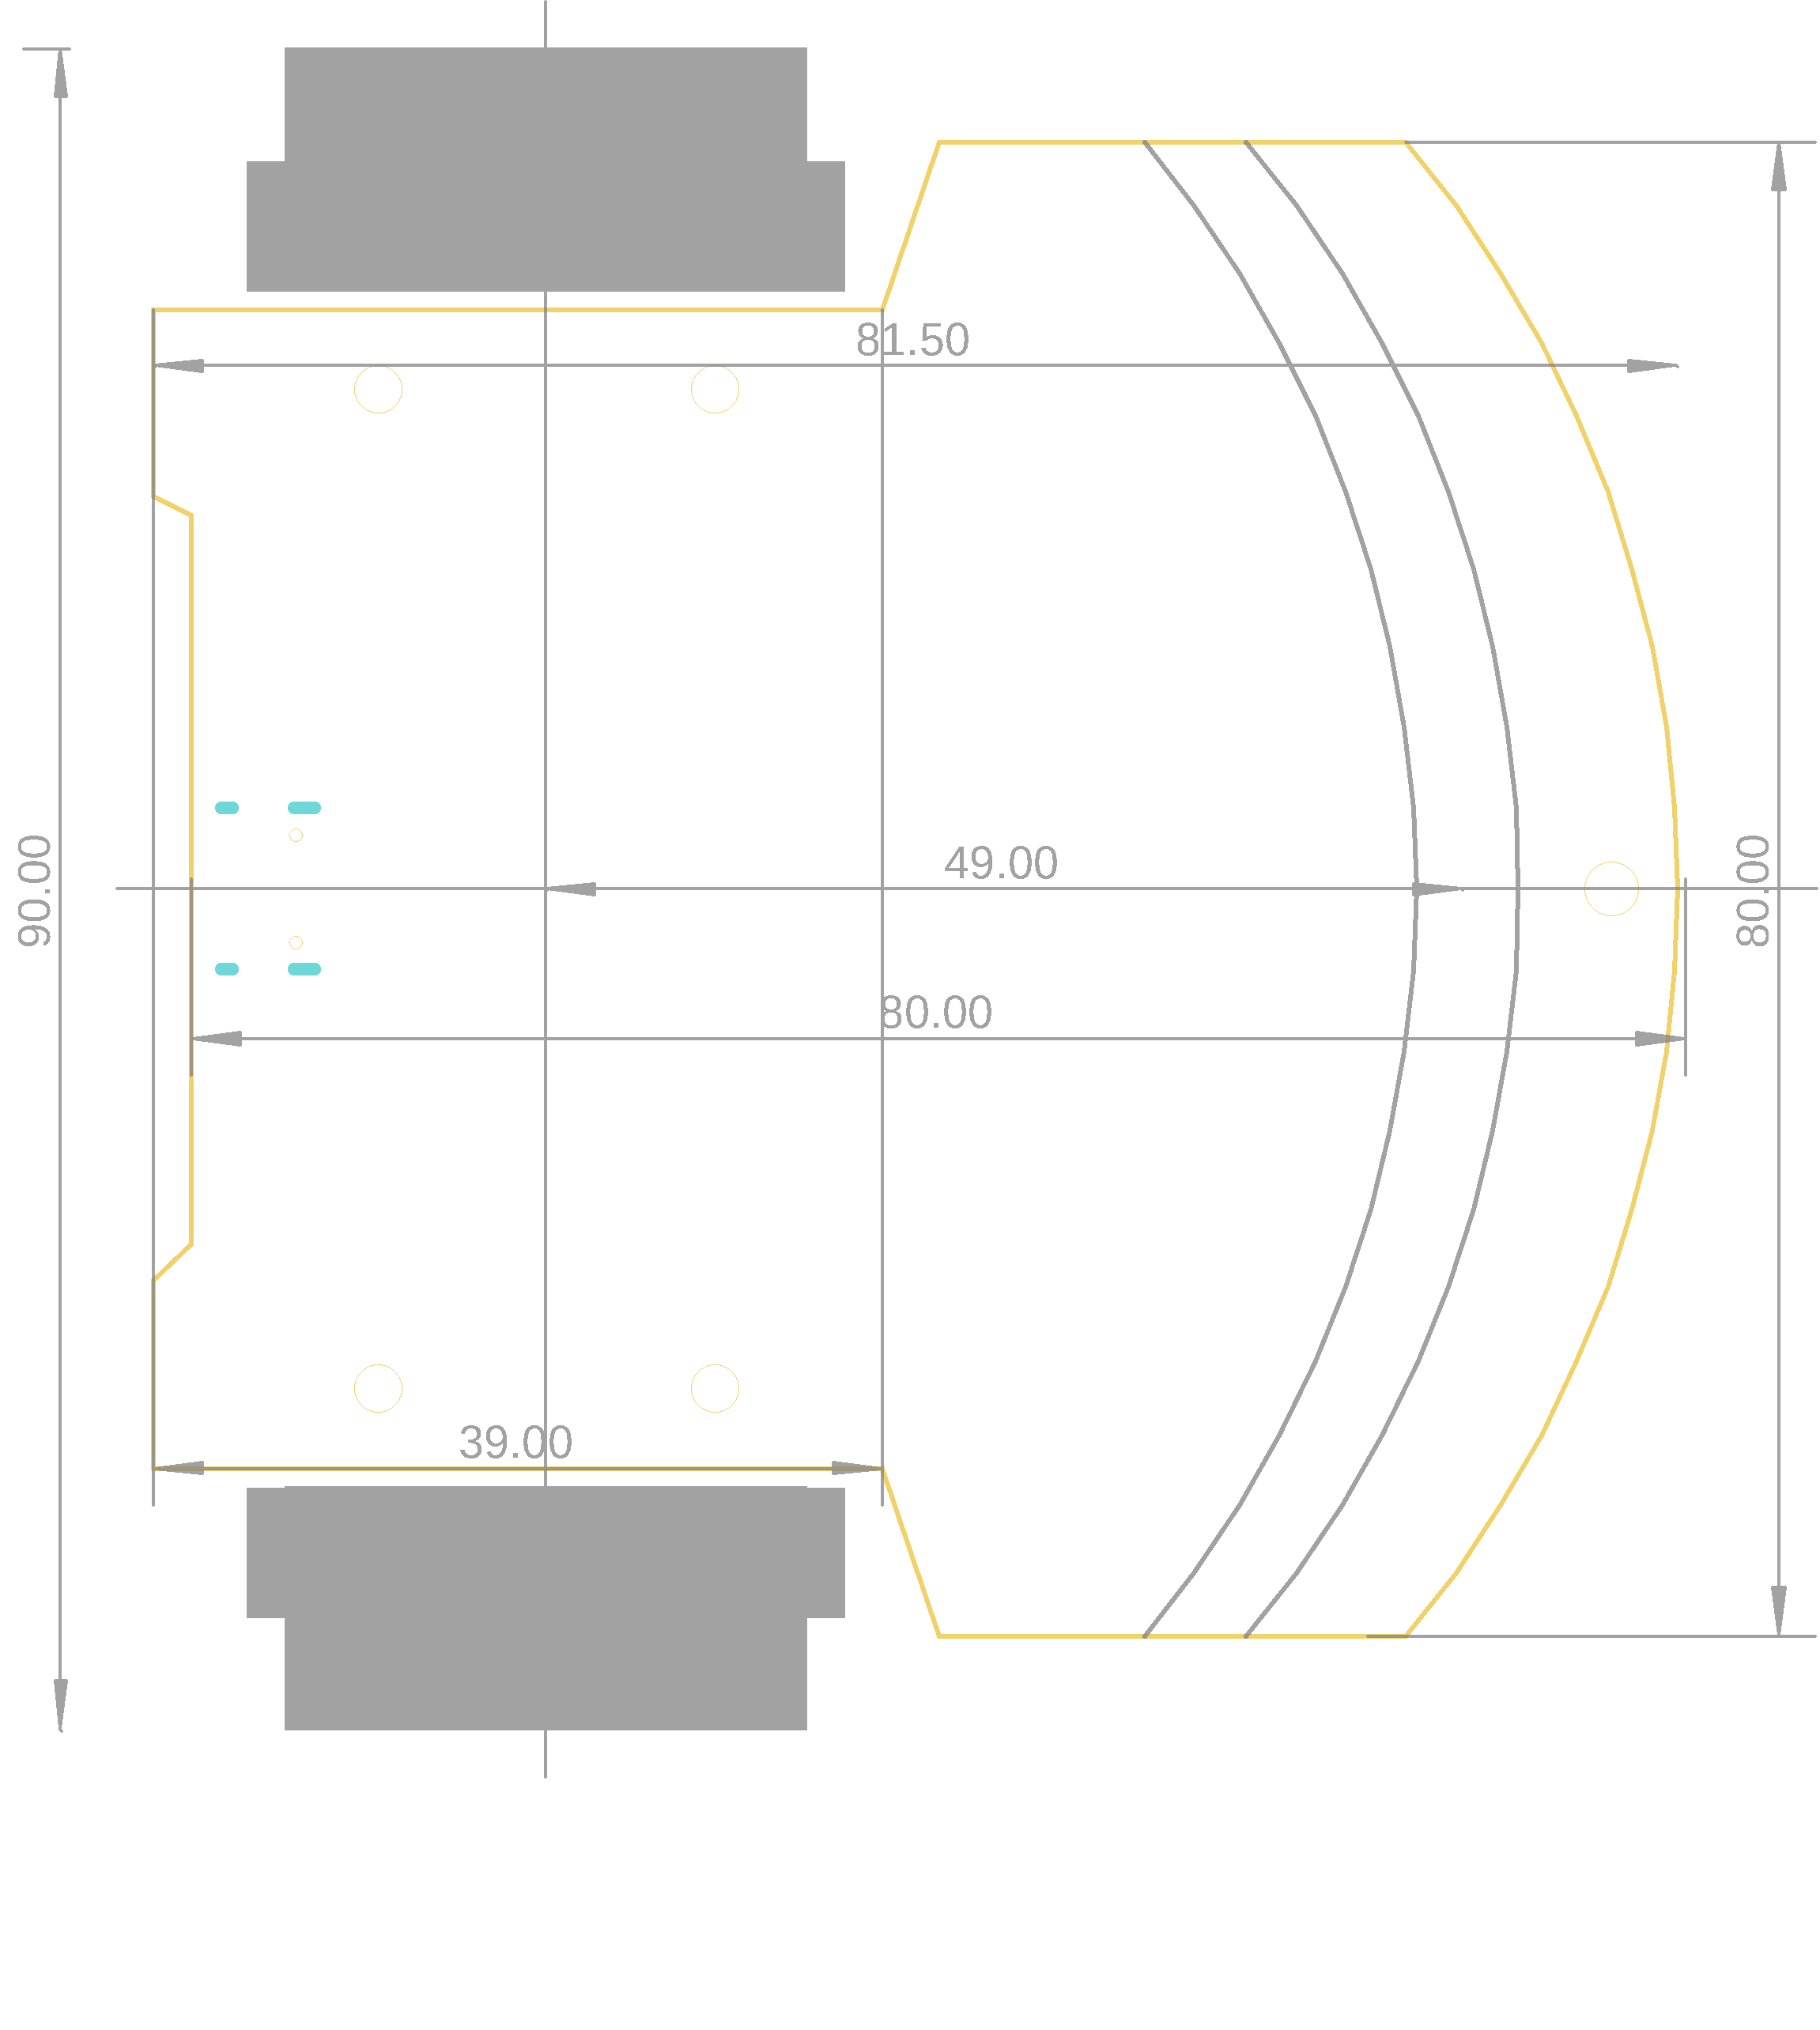
\includegraphics[scale=0.35]{../images/robot/board_dims_a.png}
            \caption{mechanical dimensions}
            \label{fig:mechanical_dimensions}
        \end{subfigure}%
        \begin{subfigure}{.5\textwidth}
            \centering
            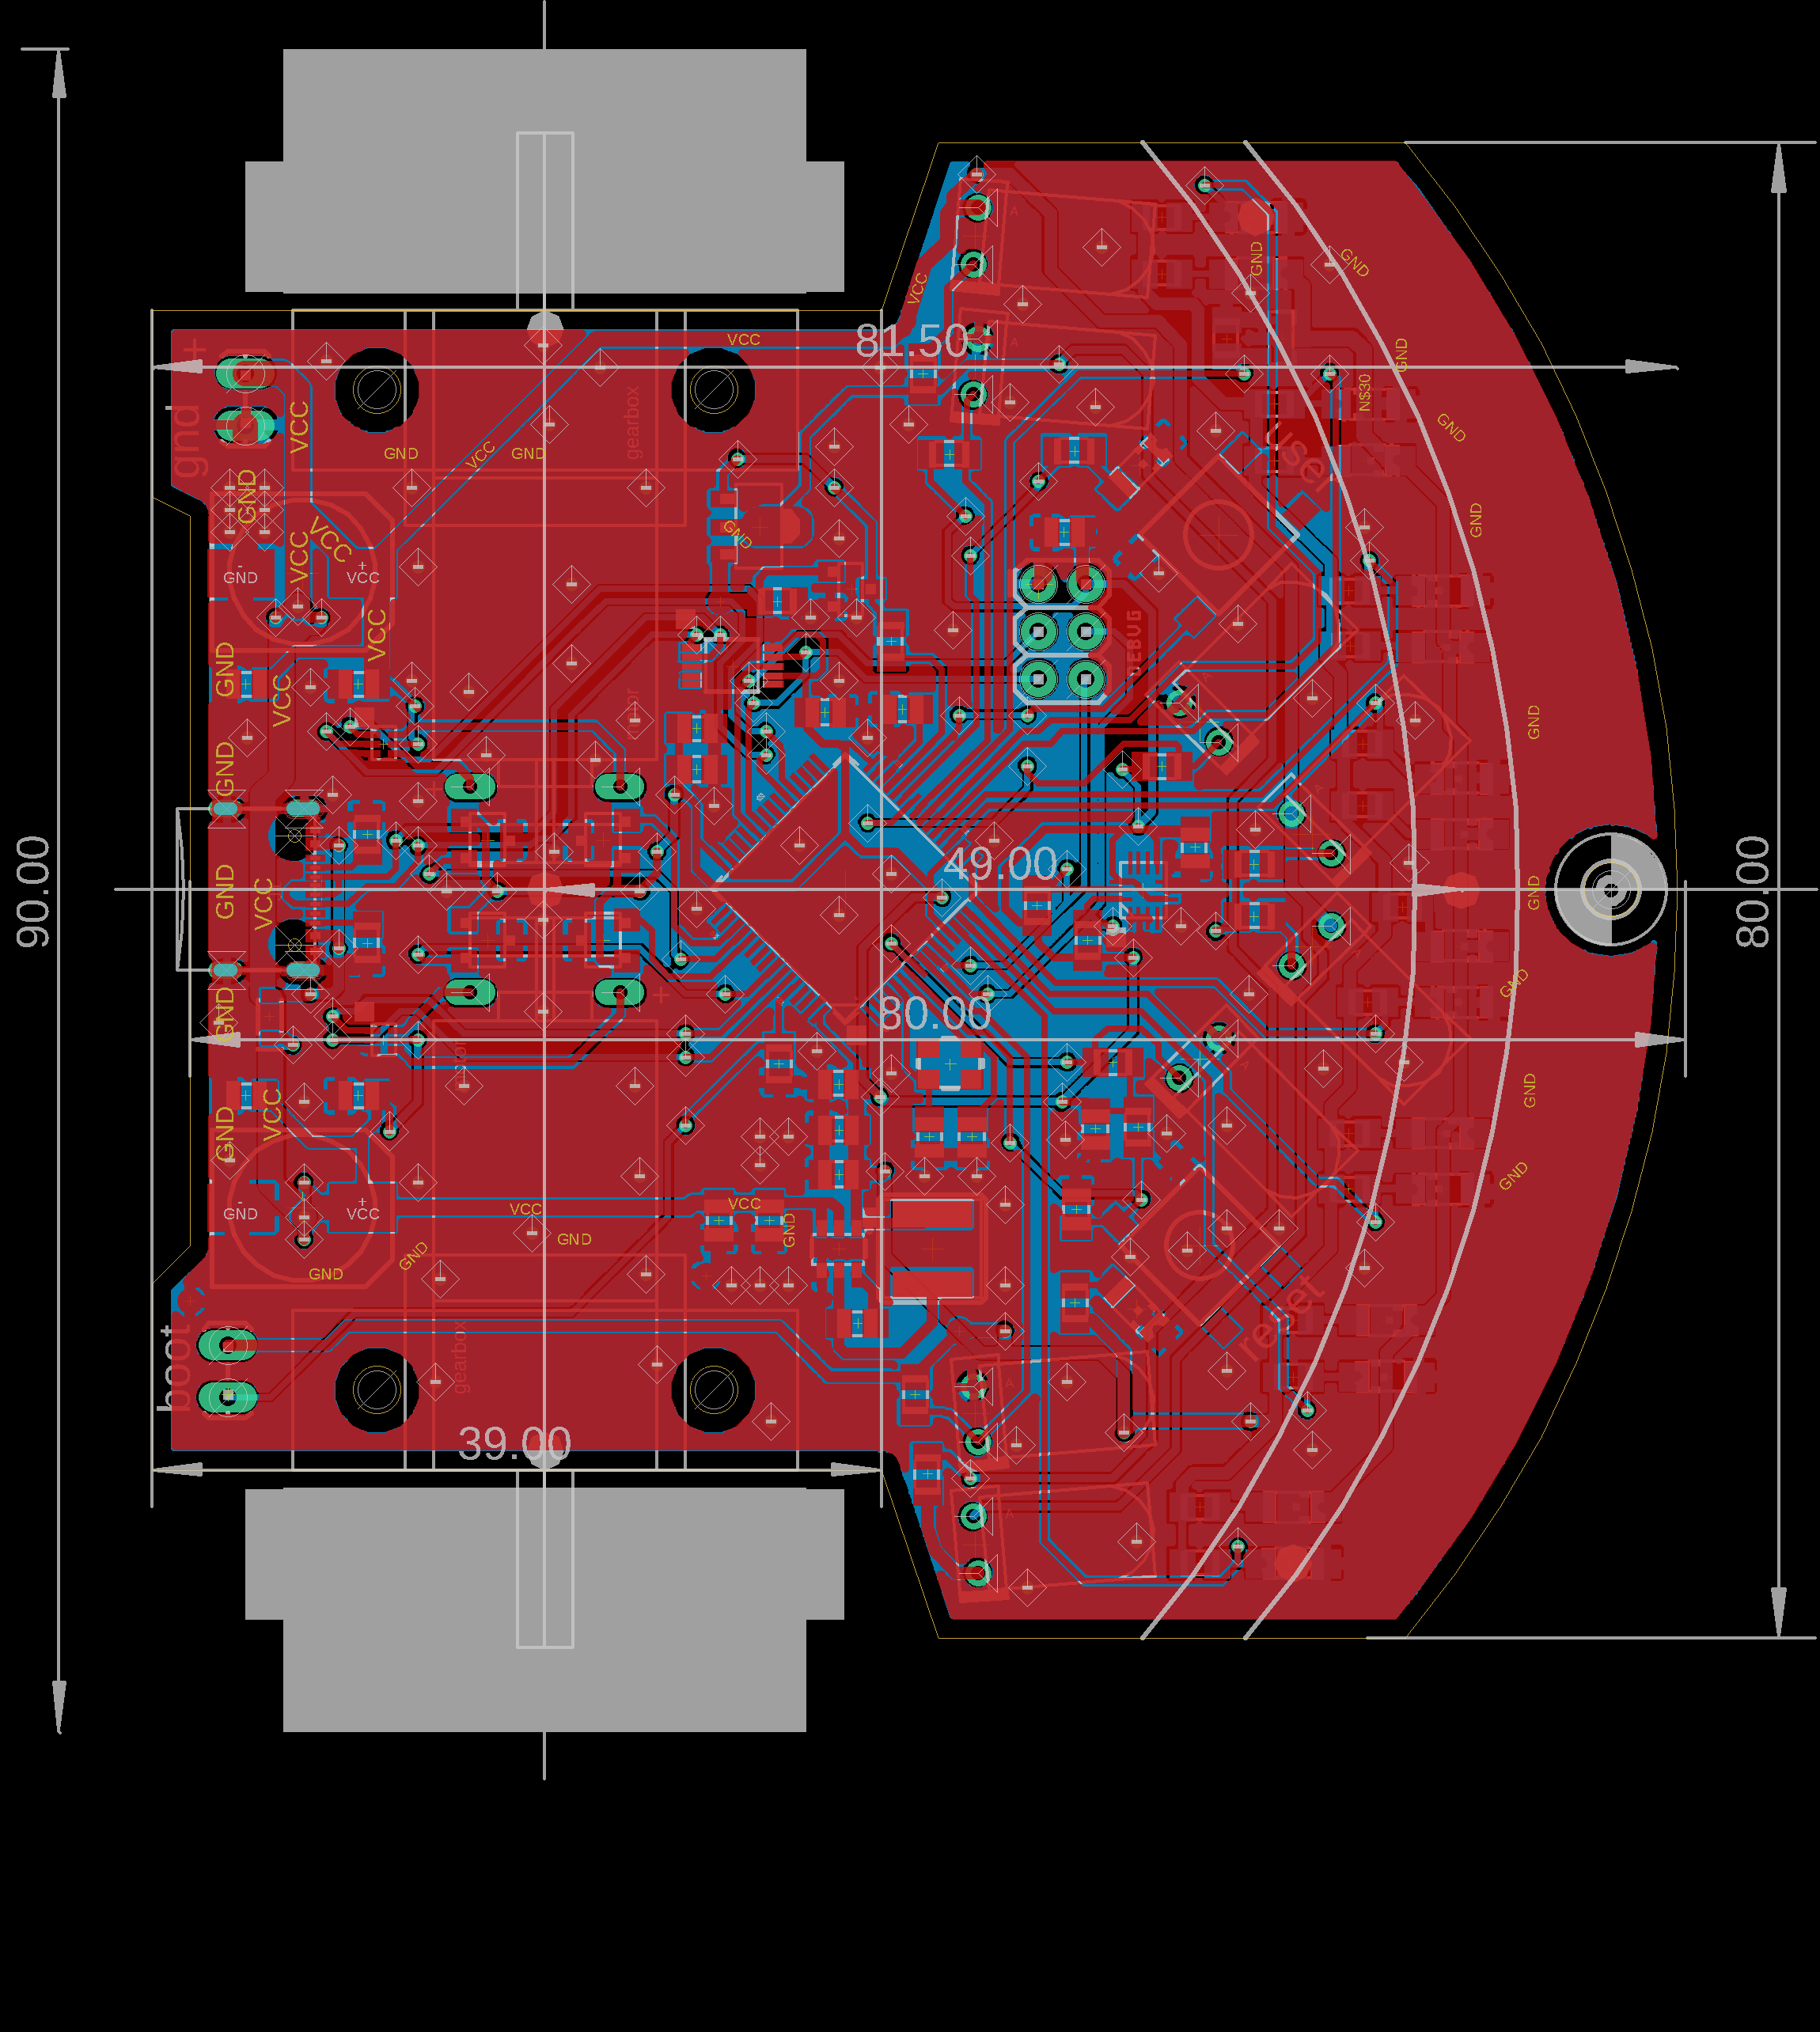
\includegraphics[scale=0.35]{../images/robot/board_all.png}
            \caption{overall PCB layout}
            \label{fig:overall_PCB_layout}
        \end{subfigure}


        \caption{Robot PCB}
    \end{figure}

    \begin{figure}[!b]
        \centering
        \includegraphics[scale=0.05]{../images/robot/robot_01.jpg}
        \caption{Robot photo}
        \label{fig:robot_photo}
    \end{figure}

    \newpage
    \begin{figure}[h]
        \centering
        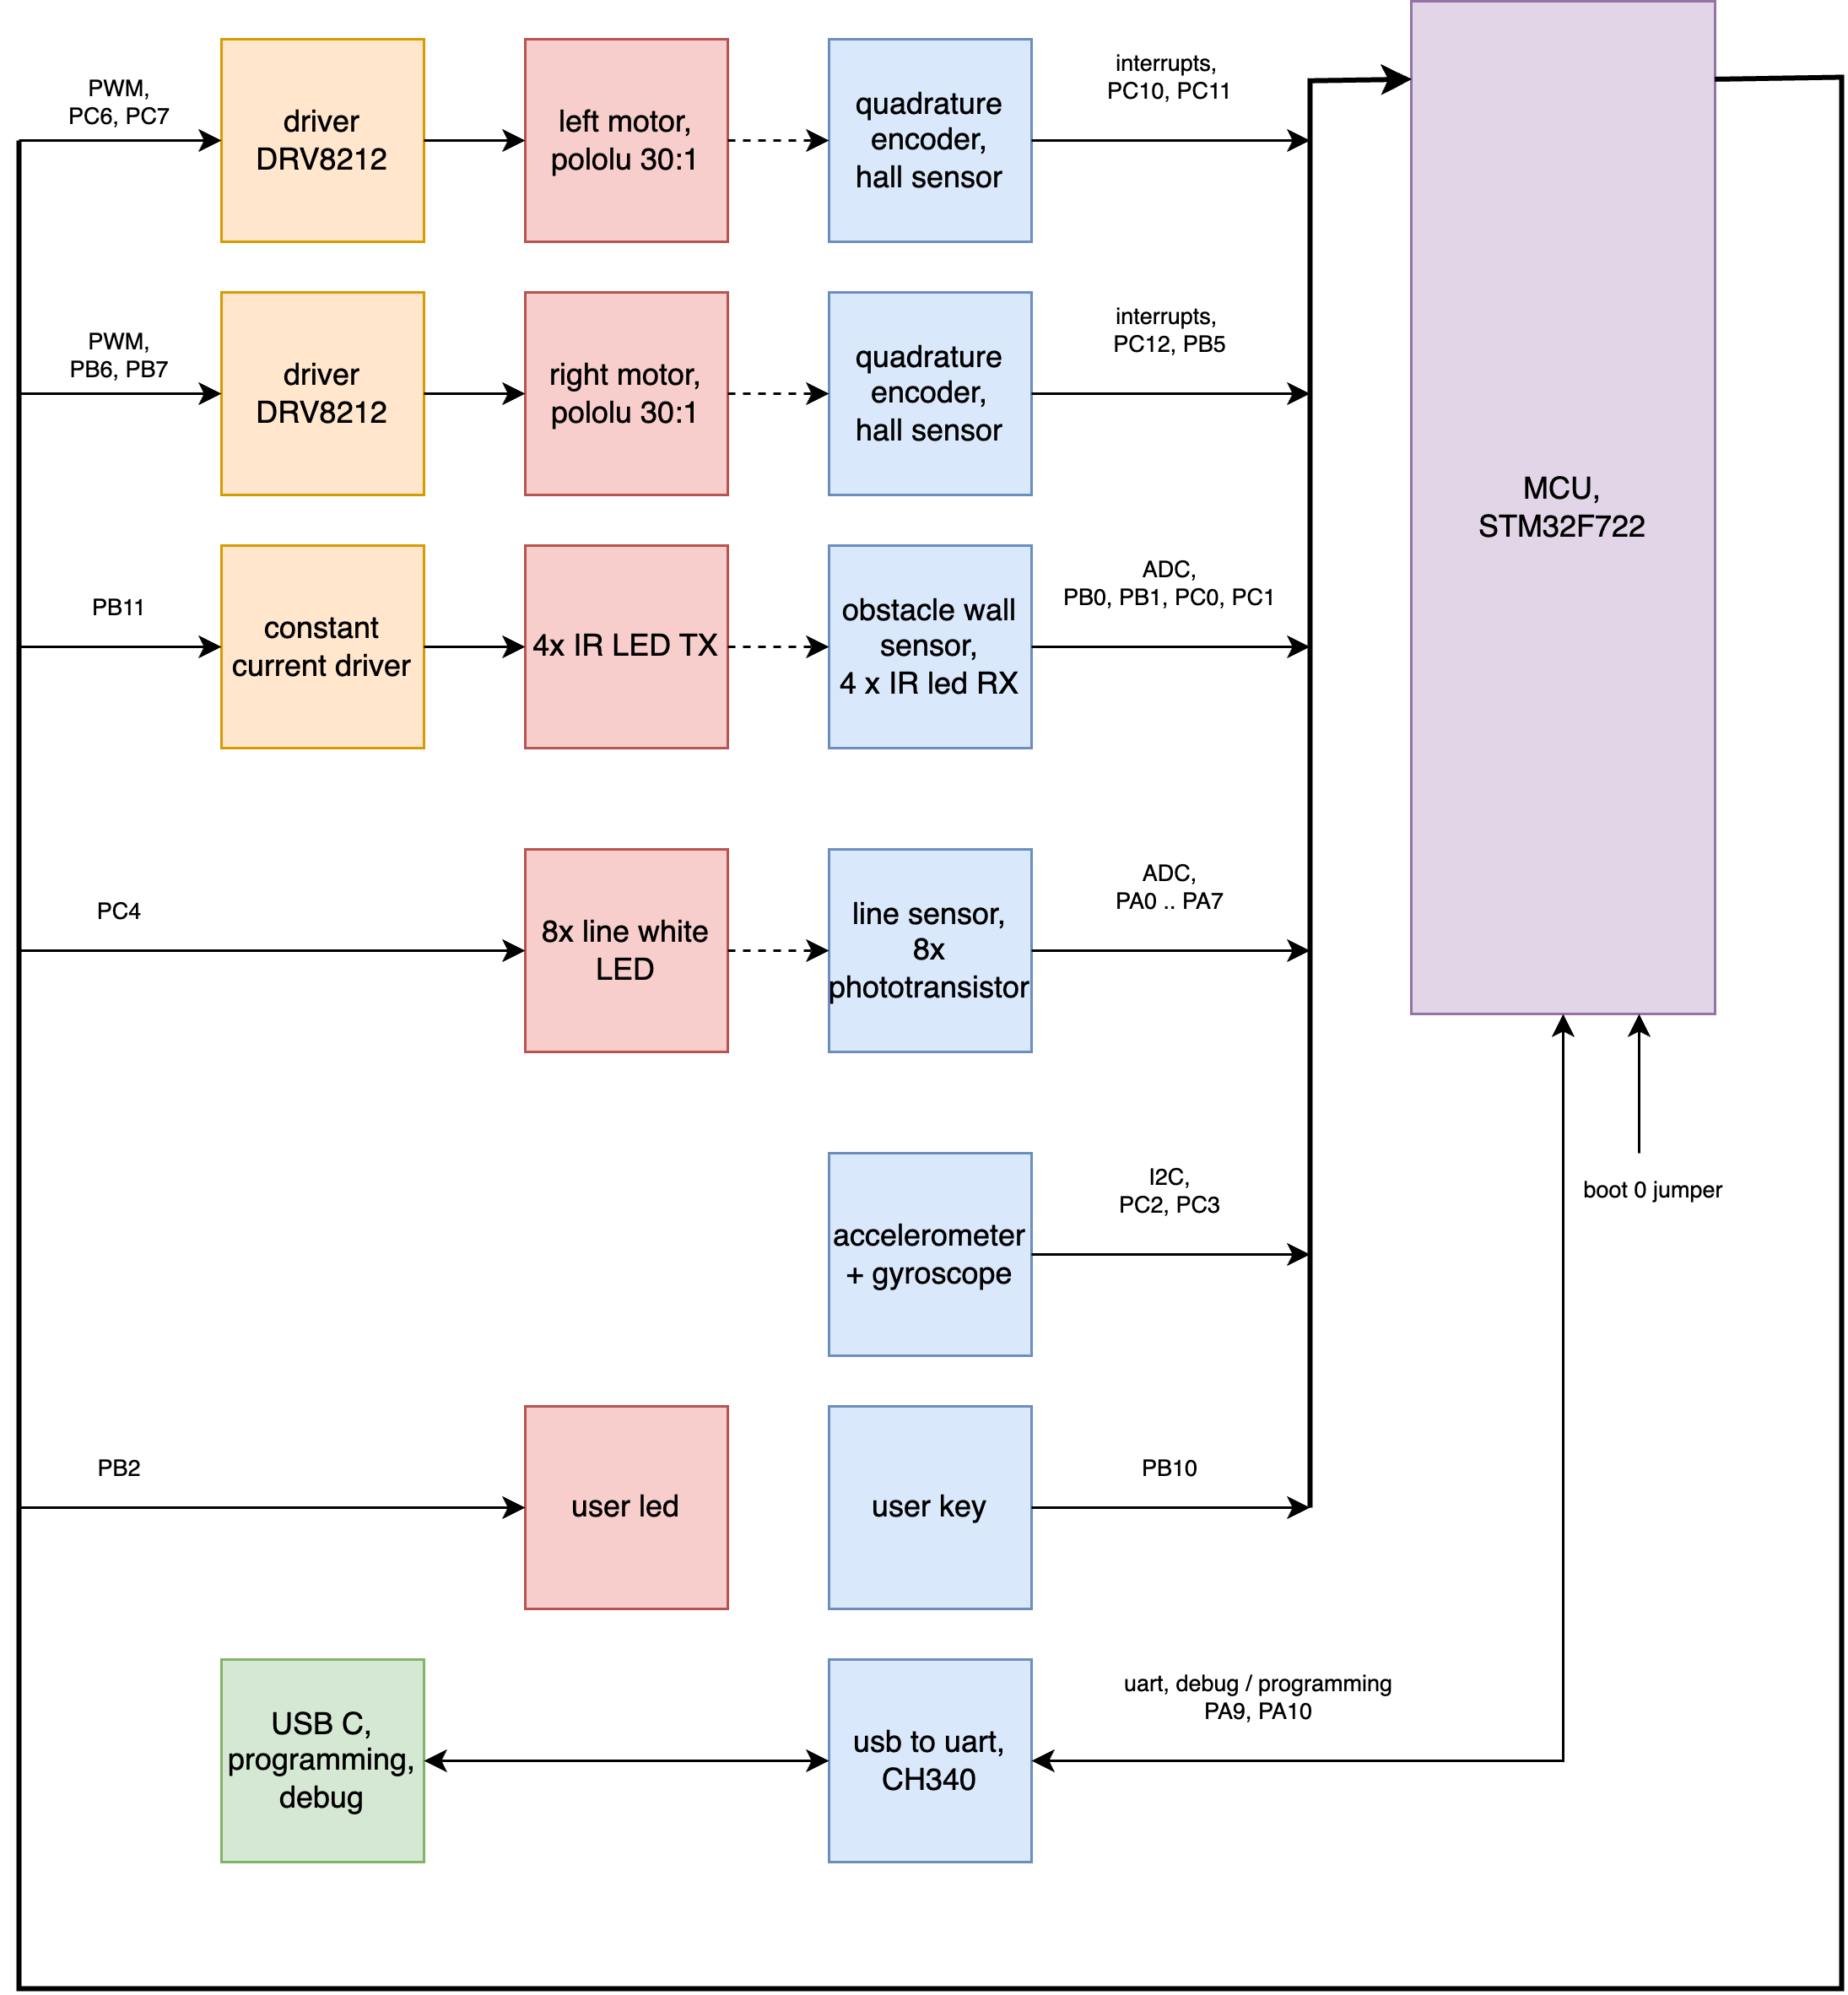
\includegraphics[scale=0.8]{../diagrams/sw/sw-block_dc.png}
        \caption{block diagram of DC motor version}
    \end{figure}

    \newpage
    \begin{figure}[h]
        \centering
        \includegraphics[scale=0.28]{../images/robot/schem_gs.png}
        \caption{schematic diagram of DC motor version}
    \end{figure}

    \newpage

        \begin{table}[h!]
            \centering
                \begin{tabular}{||c c c c c||} 
                \hline
                pin number & pin name & function & peripheral & AF number \\
                \hline\hline
                    14 & PA0 & line sensor ADC0, right & ADC1 & analog in \\ 
                    15 & PA1 & line sensor ADC1 & ADC1 & analog in \\ 
                    16 & PA2 & line sensor ADC2 & ADC1 & analog in \\ 
                    17 & PA3 & line sensor ADC3 & ADC1 & analog in \\ 
                    20 & PA4 & line sensor ADC4 & ADC1 & analog in \\ 
                    21 & PA5 & line sensor ADC5 & ADC1 & analog in \\ 
                    22 & PA6 & line sensor ADC6 & ADC1 & analog in \\ 
                    23 & PA7 & line sensor ADC7, left & ADC1 & analog in \\ 
                    & & & & \\
                    25 & PB0 & IR sensor ADC8, front left  & ADC1 & analog in \\ 
                    26 & PB1 & IR sensor ADC9, left & ADC1 & analog in \\ 
                    8 & PC0 & IR sensor ADC10, right & ADC1 & analog in \\ 
                    9 & PC1 & IR sensor ADC11, front right & ADC1 & analog in \\ 
                    & & & & \\
                    51 & PC10 & encoder left A  & GPIOC &  \\ 
                    52 & PC11 & encoder left B  & GPIOC &  \\ 
                    53 & PC12 & encoder right A  & GPIOC &  \\ 
                    57 & PB5  & encoder right B  & GPIOB &  \\ 
                    & & & & \\
                    37 & PC6 & PWM left A   & TIM3\_CH1 & AF2 \\     
                    38 & PC7 & PWM left B   & TIM3\_CH2 & AF2 \\ 
                    58 & PB6 & PWM right A  & TIM4\_CH1 & AF2 \\ 
                    59 & PB7 & PWM right B  & TIM4\_CH2 & AF2 \\ 
                    & & & & \\
                    10 & PC2 & IMU I2C, SDA & GPIOC &  \\ 
                    11 & PC3 & IMU I2C, SCL & GPIOC &  \\ 
                    & & & & \\
                    42 & PA9 & uart TX & UART1 & AF7 \\ 
                    43 & PA10 & uart RX & UART1 & AF7 \\ 
                    & & & & \\
                    27 & PB2 & user LED & GPIOB &  \\ 
                    28 & PB10 & user Key & GPIOB &  \\ 
                    29 & PB11 & IR LED control & GPIOB &  \\ 
                    24 & PC4 & line LED control & GPIOC &  \\ 
                    & & & & \\
                    7 & NRST & reset &  &  \\ 
                    60 & BOOT0 & firmware bootloader control &  &  \\ 
                \hline
                \end{tabular}
            \caption{pin mapping and function}
            \label{table:1}
        \end{table}


\chapter{Motor control}

    motor velocity controller

    \begin{figure}[!htb]
        \centering
        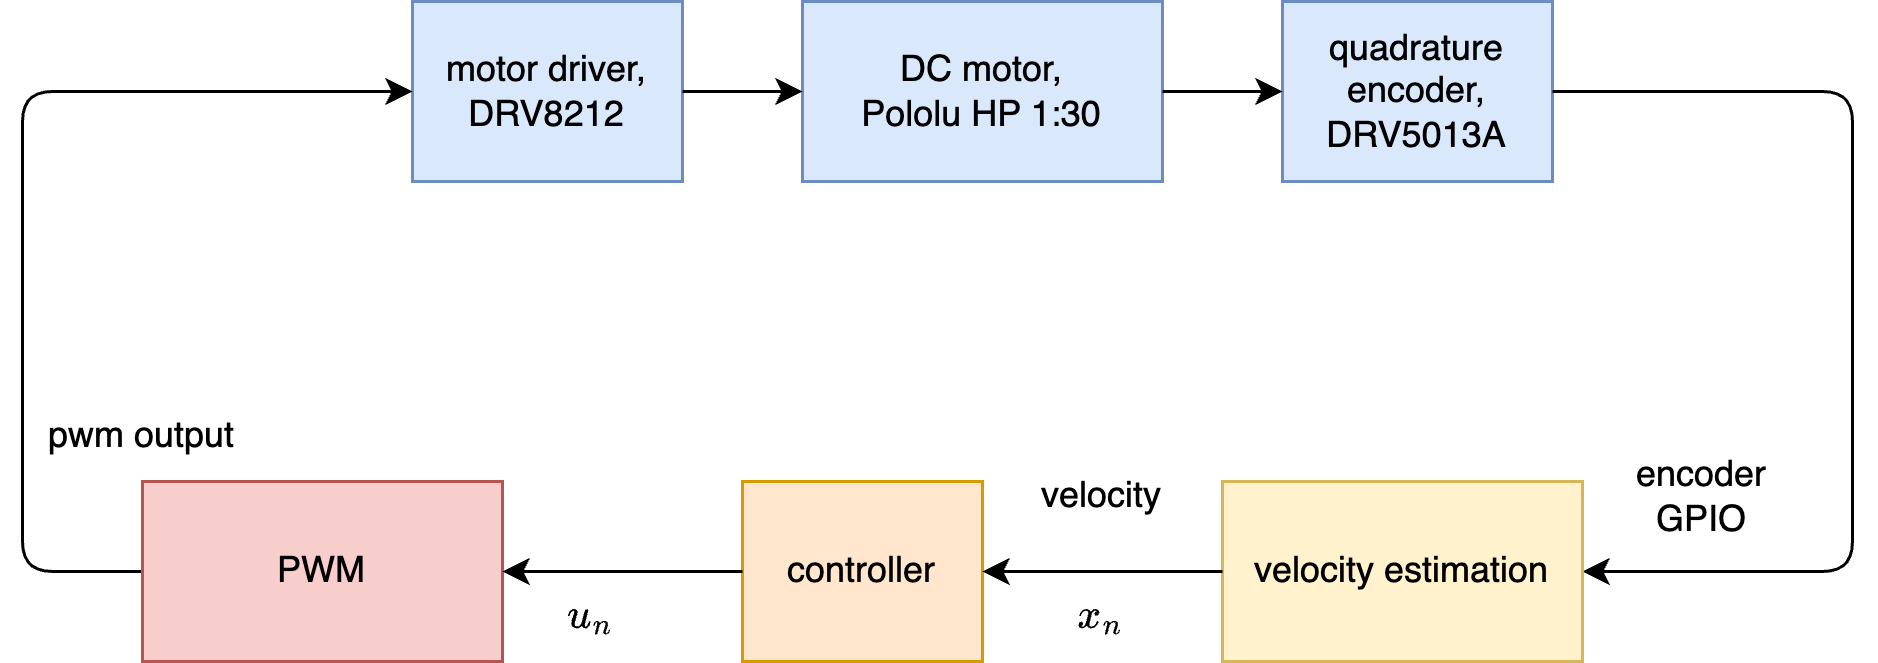
\includegraphics[scale=0.6]{../diagrams/control_generic/control_generic-motor_control.png}
        \caption{Velocity control overview}
        \label{fig:velocity_control_overview}
    \end{figure}

    \begin{figure}[!htb]
        \centering
        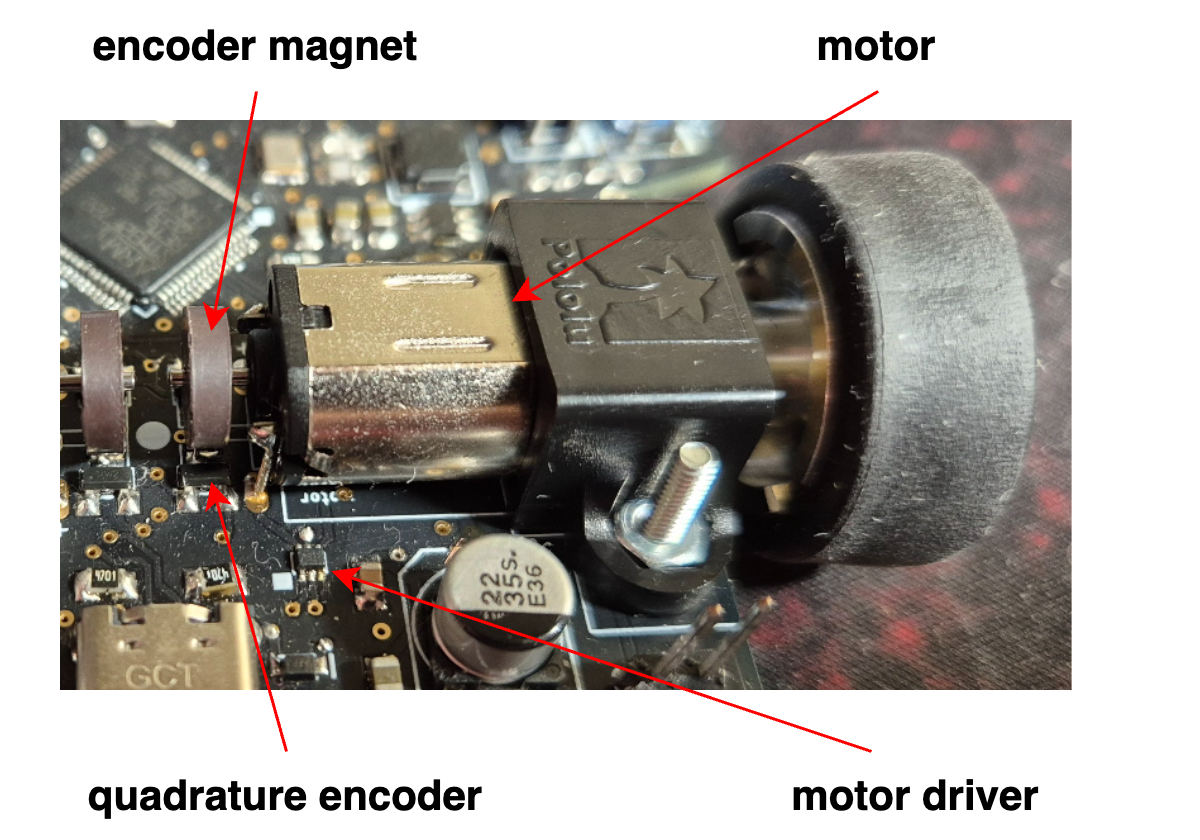
\includegraphics[scale=0.8]{../diagrams/control_generic/control_generic-motor_control_photo.png}
        \caption{Real system photo}
        \label{fig:velocity_control_real}
    \end{figure}




    \newpage
    \section{PID control}

        \begin{figure}[!htb]
            \centering
            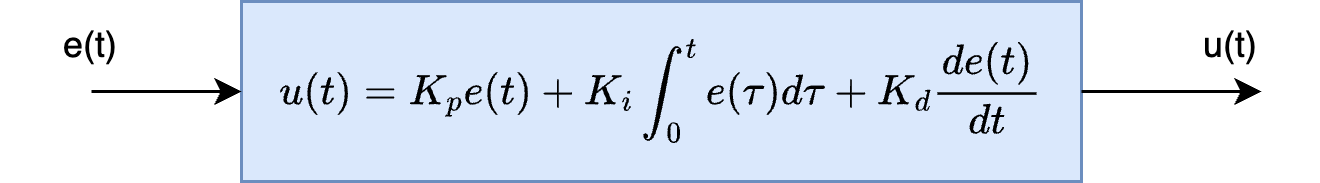
\includegraphics[scale=0.8]{../diagrams/control_generic/control_generic-pid.png}
            \caption{Textbook continuous PID controller}
            \label{fig:textbook_continuous_pid_controller}
        \end{figure}

        \begin{figure}[!htb]
            \centering
            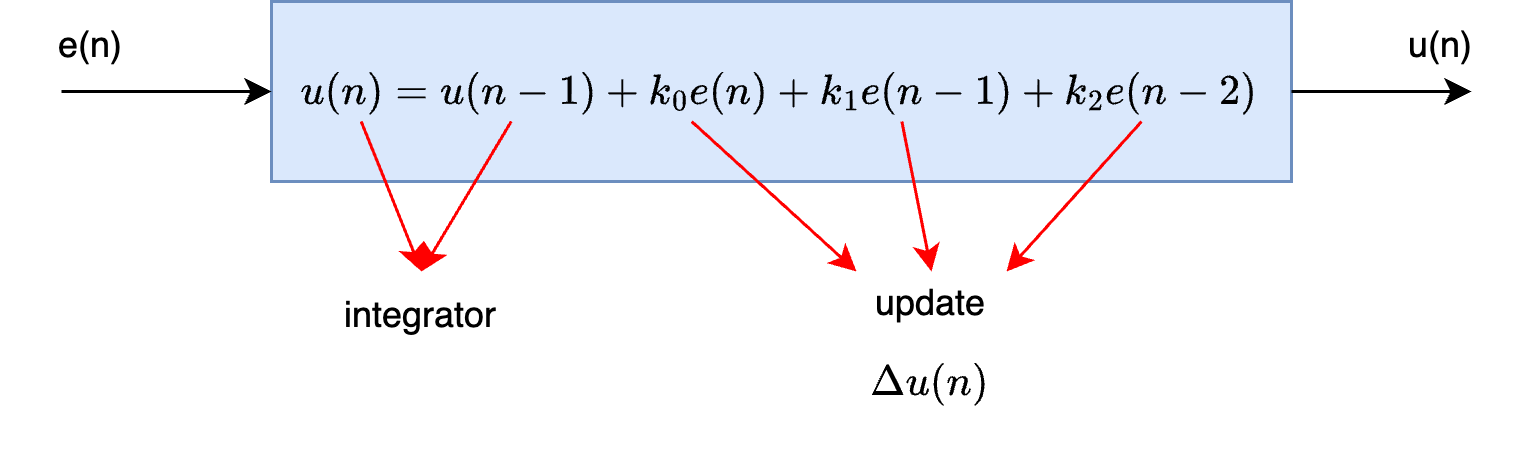
\includegraphics[scale=0.8]{../diagrams/control_generic/control_generic-pid_discrete.png}
            \caption{Discrete PID controller }
            \label{fig:discrete_pid_controller}
        \end{figure}

        
        \begin{align*}
            k_0 &= K_p + K_i\Delta t + \frac{K_d}{\Delta t} \\
            k_1 &= -K_p - 2\frac{K_d}{\Delta t} \\
            k_2 &= \frac{K_d}{\Delta t}
        \end{align*}

            \newpage
            \subsection{PID control - P only controller}

                \begin{itemize}
                    \item  target value : \textcolor{red}{\textbf { 1000rpm}}
                    \item  P-only control causes \textcolor{red}{\textbf {steady state error}}
                \end{itemize}
            
                \begin{align*}
                    u(n+1) &= u(n-1) + k_pe(n) - k_pe(n-1) \\
                    k_p    &= 0.01
                \end{align*}

                \begin{figure}[!htb]
                    \centering
                    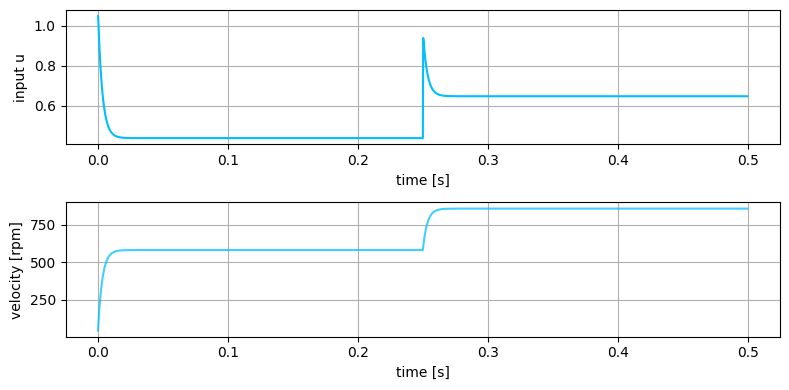
\includegraphics[scale=0.8]{../images/motor_control/pid_p_control.png}
                    \caption{P-only controller}
                    \label{fig:p_controller}
                \end{figure}

            \newpage
            \subsection{PID control - PI}
                
                too high I term 

                \begin{itemize}
                    \item  target value : \textcolor{red}{\textbf {1000rpm}}
                    \item  PI control \textcolor{red}{\textbf {removes steady state error}}
                    \item  too high I term causes \textcolor{red}{\textbf {oscilations and overshot}}
                \end{itemize}
            
              
                \begin{align*}
                    u(n+1) &= u(n-1) + (k_p + k_i\Delta t) e(n) - k_pe(n-1) \\
                    k_p    &= 0.01 \\
                    k_i    &= 0.005
                \end{align*}
                
                
                \begin{figure}[!htb]
                    \centering
                    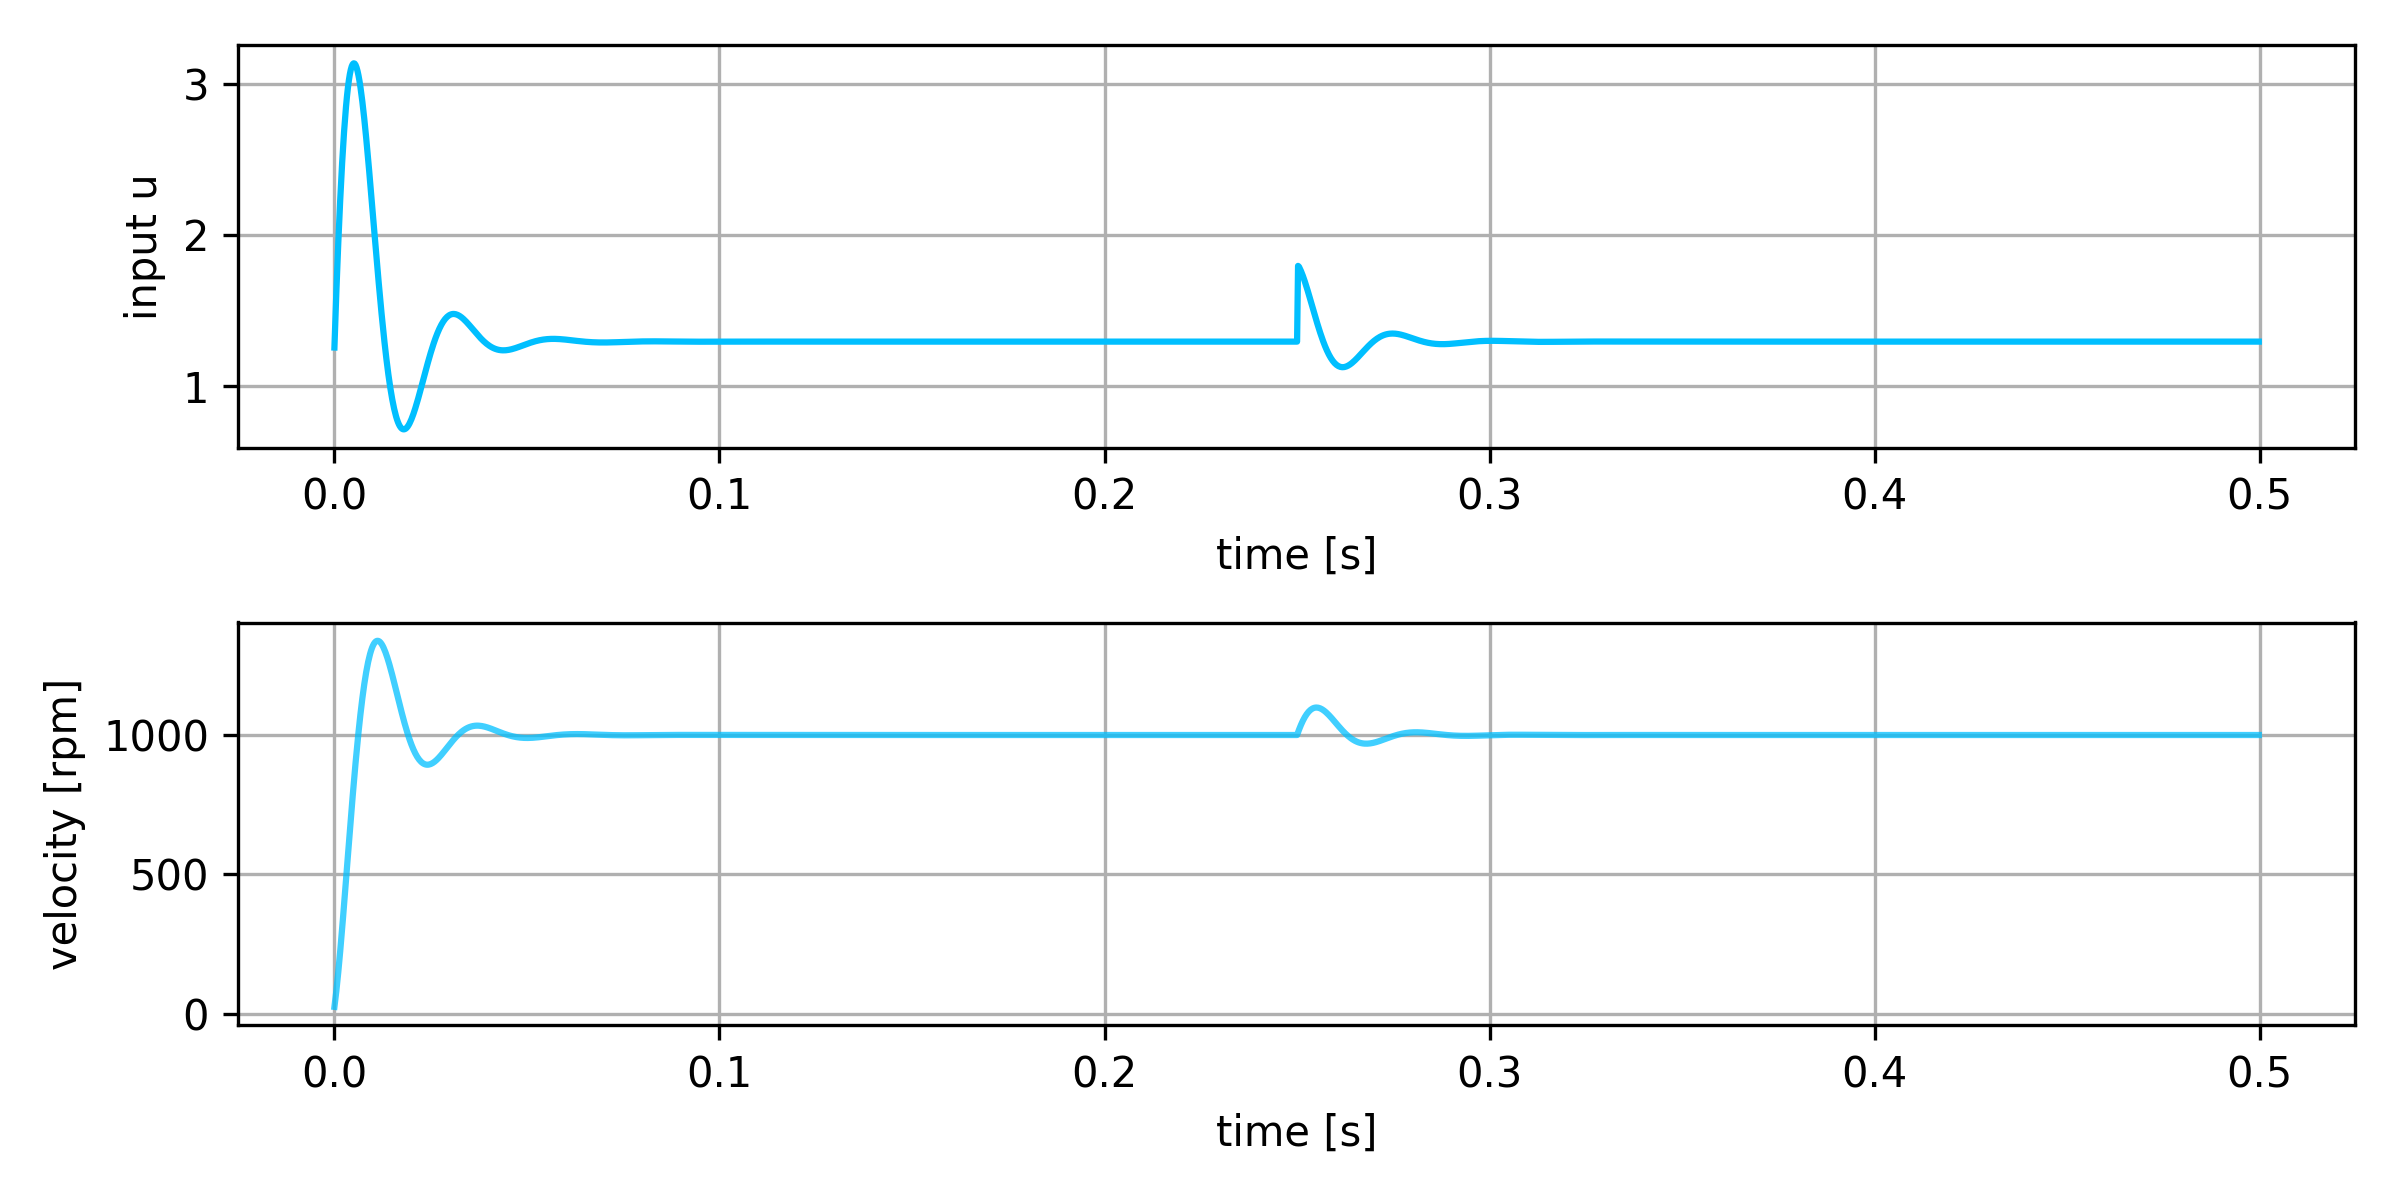
\includegraphics[scale=0.8]{../images/motor_control/pid_pi_control_0.png}
                    \caption{PI controller}
                    \label{fig:pi_controller}
                \end{figure}

                correct I term

                \begin{itemize}
                    \item  target value : \textcolor{red}{\textbf {1000rpm}}
                    \item  correct tunned PI controller for 1st order system
                    \item  \textcolor{red}{\textbf {no overshot, no steady state error}}
                \end{itemize}
                
                \begin{align*}
                u(n+1) &= u(n-1) + (k_p + k_i\Delta t) e(n) - k_pe(n-1) \\
                k_p    &= 0.01 \\
                k_i    &= 0.0002
                \end{align*}

                \begin{figure}[!htb]
                    \centering
                    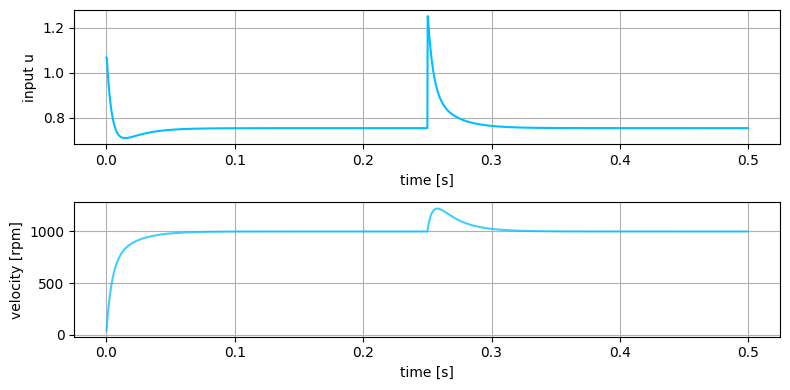
\includegraphics[scale=0.8]{../images/motor_control/pid_pi_control_1.png}
                    \caption{PI controller with correct parameters}
                    \label{fig:pi_controller_correct}
                \end{figure}
                
            \newpage
            \subsection{complete discrete PID algorithm}  
    
                \begin{enumerate}
                  \item  calculate u-change candidate :
                    $$\Delta \hat{u}(n) = k_0e(n) + k_1e(n) + k_2e(n)$$
                  
                  \item clip maximum allowed u-change, to avoid u-kick :
                    $$\Delta u(n) = clip(\Delta \hat{u}(n), -du_{min}, du_{max})$$
              
                  \item clip maximum allowed u value, to avoid saturation / windup :
                    $$u(n) = clip(u(n-1) + \Delta u(n), -u_{min}, u_{max})$$
                \end{enumerate}

                \begin{figure}[!htb]
                    \centering
                    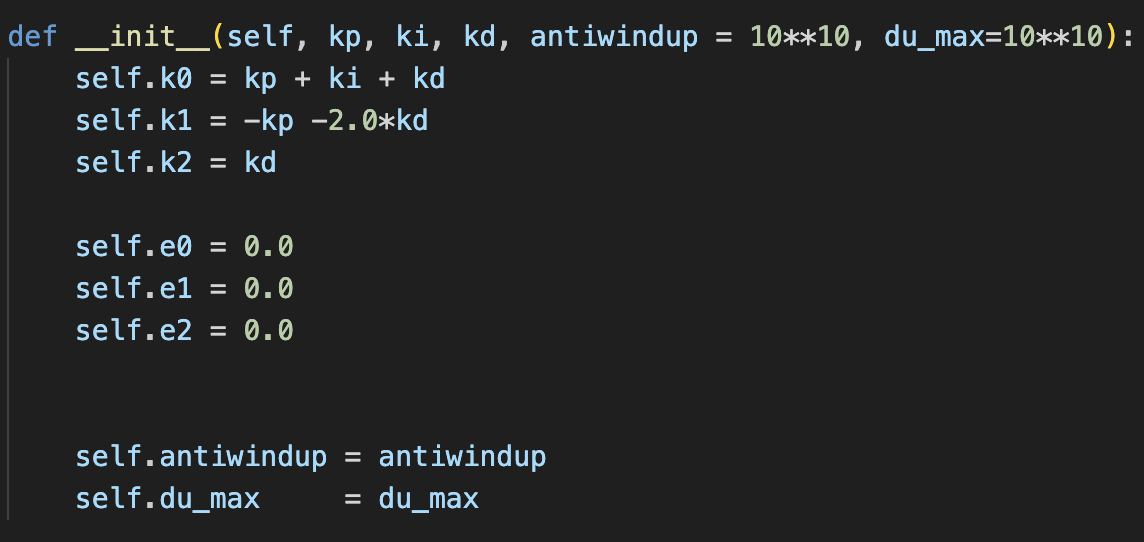
\includegraphics[scale=0.8]{../images/control/pid_init.png}
                    \caption{Initialisation}
                    \label{fig:code_discrete_pid}
                \end{figure}

                \begin{figure}[!htb]
                    \centering
                    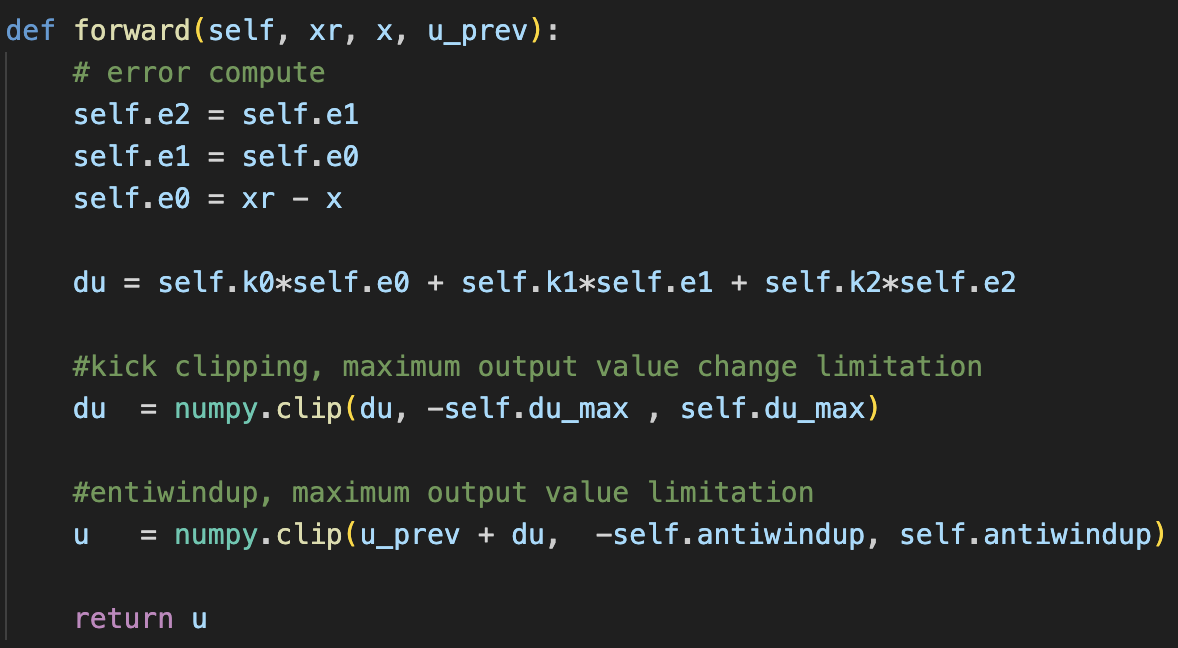
\includegraphics[scale=0.8]{../images/control/pid_main.png}
                    \caption{Main loop}
                    \label{fig:code_discrete_pid}
                \end{figure}


  

\end{document}